\documentclass[10pt]{article}
\usepackage[utf8]{inputenc}
\usepackage[T1]{fontenc}
\usepackage[italian]{babel}

\usepackage{geometry}
\geometry{a4paper}

\usepackage{fancyhdr}
\pagestyle{fancy}
\renewcommand{\headrulewidth}{0pt}
\lhead{}\chead{}\rhead{}
\lfoot{}\cfoot{\thepage}\rfoot{}

\usepackage{graphicx}
\usepackage{booktabs}
\usepackage{paralist}
\usepackage{verbatim}
\usepackage{subfig}

\usepackage{sectsty}

\usepackage[titles,subfigure]{tocloft}
\renewcommand{\cftsecfont}{\rmfamily\mdseries\upshape}


\title{ADC DAC GPIO Board for Raspberry}
\author{Patrick Predella 165283, Federico D'Eredità 151646 }
\date{}

\begin{document}
\maketitle
\tableofcontents

\section{Introduzione}
% Breve spiegazione della finalità del progetto e metodo usato per giungere a tal fine
Finalità del progetto è il monitoraggio di misure di temperatura e pressione ambientali mediante sensoristica analogica con la possibilità di comandare attuatori analogici e/o digitali tramite programmazione di un Raspberrt Pi2+.
A questo scopo abbiamo deciso di realizzare una scheda composta dai seguenti elementi principali:
\begin{itemize}
\item Un convertitore analogico-digitale per il campionamento dei segnali analogici di temperatura e pressione affiancato da una protezione per eventuali sbalzi di tensione;
\item Un convertitore digitale-analogico per il controllo di attuatori analogici anch'esso affiancato da una protezione per eventuali sbalzi di tensione;
\item Un general purpose input/output per il controllo di attuatori digitali ed il controllo delle operazioni pre-programmate nel Raspberry;
\item Scheda PiggyBack (vedasi capitolo \ref{sec:piggy}) per l'assemblaggio della componentistica;
\item Un Raspberry Pi2+ per il controllo delle linee dati, di clock e l'interazione con il GPI/O.
\end{itemize}


\section{Componentistica}
	\subsection{Cicuiteria utilizzata}

		\subsubsection{ADC - Analog-to-Digital Converter}\label{sec:adc}
		% Breve introduzione
%		- Cos'è un ADC (genericamente) e come funziona (frequenza di campionamento, vref e breve cenno all campionamento differenziale)
%		- L'MCP xxxx (nel dettaglio), schema, pin e loro descrizione, max ratings, PGO
%		- Come NOI lo colleghiamo ai sensori, spiegazione Ch+ Ch- e perchè è un campionamento differenziale.
		L'ADC è un dispositivo per la conversione di segnali analogici in segnali digitali, i suoi aspetti più importanti sono risoluzione e frequenza di campionamento.
		La risoluzione è legata al numero di bit di memoria disponibili nel dispositivo e influenza la sua capacità di discernere segnali in ingresso simili tra loro mediante $2^{n-1}$ step di campionamento (con n pari al numeri di bit disponibili). La frequenza di campionamento invece determina in che misura la conversione segua fedelmente l'andamento nel tempo del segnale di ingresso. Come noto dal teorema di Shannon la frequenza di campionamento deve essere almeno più del doppio della frequenza del segnale ingresso, nel caso in esame comunque i segnali di temperatura e pressione essento riferiti a misure ambientali hanno frenquenze molto basse.
		
		Nel nostro progetto utilizziamo un MCP3428 della Microchip Technology Inc. caratterizzato da una frequenza di lavoro a 100 kHz, 400 kHz o 3.4 MHz (nella nostra applicazione imposteremo 100 kHz) ed una risoluzione a 16bit e 4 canali d'ingresso. In figura \ref{fig:adc} è possibile vedere una schematizzazione a blocchi del funzionamento dell'ADC in uso.
		\begin{figure}[h]
		\centering
		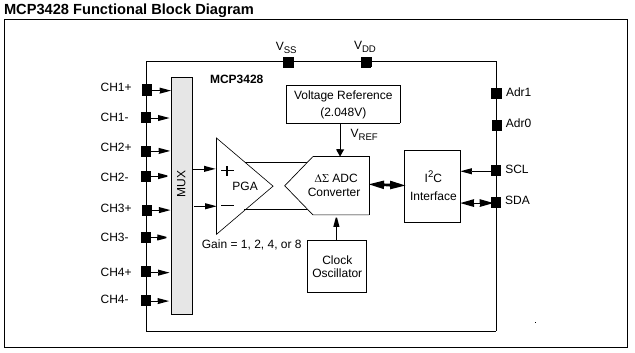
\includegraphics[width=0.8\textwidth]{src/adc_block}
		\caption{Schema a blocchi dell'ADC}\label{fig:adc}
		\end{figure}
		\subsubsection{DAC - Digital-to-Analog Converter}\label{sec:dac}
		% Come per ADC

		\subsubsection{GP I/O - General Purpose Input/Output Device}\label{sec:gpio}
		% Come per ADC

		\subsubsection{DCDC Converter}\label{sec:dcdc}
		Il DCDC è un componente che converte una tensione in continua in un'altra tensione in continua secondo i suoi parametri di datasheet.
		L'alimentazione verrà formita da un alimentatore da 12VDC. Tuttavia la nostra scheda monta componentistica che richiede una alimentazione a 5VDC. Usiamo quindi un DCDC converter sia per abbassare la tensione a quella desiderata che per eliminare oscillazioni dovute a eventuali picchi in ingresso

		Utilizziamo il componente LM2596. Un DCDC con Vin tra 10V e 40V e Vout stabilizzata a 5V con tolleranza \(<\)0.1\%, il che è tollerabile con tutti i nostri Absolute maximum ratings (5\(\pm\)0.005V).
		Questo componente presenta pure una linea di Feedback in modo da poter regolare in closed-loop la tensione in uscita (nel caso in cui questa sia separata da un filtro per esempio).
		Aggiungiamo quindi un condensatore in ingresso e un filtro in uscita per smorzare le tensioni entranti ed uscenti e quindi evitare eventuali glitch nelle alimentazioni dei componenti digitali.

	\subsection{Ulteriori Componenti Hardware}
		\subsubsection{La scheda Piggy-Back}\label{sec:piggy}
		% Cos'è, perché la usiamo, cenni sul numero di pin sequenziali, compatibilità col Raspberry, montaggio Circuiteria
		% - Il DCDC, schema e cenni sul closed-loop feedback -> garanzia di Vdd costante

		\subsubsection{Il Raspberry}\label{sec:rasp}
		% Massimo 3 righe su cos'è giusto per avere una descrizione a prova di idiota
		% - Collegamento e comunicazione col Piggy-Back

	\subsection{Il linguaggio di programmazione I2C}\label{sec:i2c}
	% Breve cenno sull'I2C che viene usato per la comunicazione con la circuiteria

\section{Realizzazione del Progetto}
		Il progetto è molto semplice. Si tratta di:
		\begin{itemize}
		        \item utilizzare il DCDC converter per stabilizzare l'alimentazione dei componenti.
		        \item portare le piste a degli header in modo che siano accessibili al Raspberry
		        \item proteggere le linee in ingresso e in uscita in modo che non si danneggino i componenti
		\end{itemize}

	\subsection{Protezione della componentistica}
		Si tratta di rispettare le specifiche di absolute maximum ratings, proteggere le linee in ingresso e in uscita da ingressi \textbf{out of range} e \textbf{ridurre i rumori}.
		In particolare un filtro per i rumori nel caso dell'ADC, un filtro per avere un transitorio non nullo nel caso dei GPIO e in tutti e tre i casi una protezione contro ingressi alti e per rientrare negli Absolute Maximum ratings nel caso di collegamento dei pin di output a massa (caso peggiore).
		(Vedi lo schematico delle parti: RASP\_GPIO\_DAC\_ADC\_PARTS.pdf)
		\subsubsection{Filtri RC}
		Abbiamo disegnato due filtri RC:
		\begin{itemize}
		        \item Filtro ADC.
		        \item Filtro GPIO
		\end{itemize}
		Si tratta in entrambi i casi di filtri passa basso con 1 unico polo.
			\paragraph{Filtro ADC}
				L'ADC da specifiche si comporta come un passa basso a 5hz. Nel nostro caso vogliamo aggiungere un ulteriore polo in modo da \textbf{pre-filtrare} il segnale in ingresso.
				Scegliamo quindi una frequenza di taglio \textbf{\(<\)5Hz} (sopra alla quale in ogni caso il segnale non viene campionato correttamente).
				In particolare scegliamo una resistenza da 100k\(\Omega\) e un condensatore da 1\(\mu\)F per avere di conseguenza un taglio a 1.6Hz.
			\paragraph{Filtro GPIO}
				Per il GPIO il caso è diverso: ci serve un filtro in modo da evitare false letture dovute a picchi improvvisi e rumore e nel contempo asssicurare una buona reattività nel caso dell'attuazione
				Dimensioniamo il filtro a partire dalla resistenza che deve soddisfare la massima corrente di drain dal piedino descritta negli \textbf{Absolute Maximum Ratings}.
				Abbiamo quindi Imax=25mA, Vmax=5V. Rmin deve quindi essere Rmin=200\(\Omega\). La dimensioniamo ad 1k\(\Omega\) e siamo sicuri di essere nei ratings.
				Scegliamo una C=1\(\mu\)F per avere di conseguenza un taglio a 160Hz. La porta ha quindi una \(\tau\)=1ms di risposta naturale, che è accettabile nel nostro caso perché nel caso peggiore la commutazione del valore binario avviene intorno ai 2ms.
		\subsubsection{Protezioni V e I}
		Ci serve un sistema per impedire alla tensione di salire oltre ad una certa soglia in modo da non danneggiare i microchip. utilizziamo quindi dei diodi zener che scaricano a massa le tensioni in ingresso.
		Si noti che le usiamo anche nel caso dei DAC per proteggere la porta nel caso in cui venga collegata erroneamente.
			\paragraph{Protezione DAC}
				Nel caso del DAC vogliamo proteggere la porta da tensioni troppo alte. Al massimo il DAC da Vout=Vdd=5V. Colleghiamo un diodo Zener con Vz=5.1V in inversa e qualunque tensione maggiore di 5.1 verrà scaricata dal componente.
				La resistenza viene scelta per rispettare la massima corrente erogata dal pin Imax=25mA. Con V=5V e Imax=25mA, Rmin=200\(\Omega\). La dimensioniamo ad 1k\(\Omega\).
			\paragraph{Protezione GPIO}
				Pure nel caso del GPIO vogliamo proteggere la porta da tensioni troppo alte. Al massimo il GPIO da Vout=Vdd=5V. Colleghiamo un diodo Zener con Vz=5.1V in inversa e qualunque tensione maggiore di 5.1 verrà scaricata dal componente.
				La resistenza viene scelta per rispettare la massima corrente erogata dal pin Imax=25mA. Con V=5V e Imax=25mA, Rmin=200\(\Omega\). La dimensioniamo ad 1k\(\Omega\).
			\paragraph{Protezione ADC}
				Nel caso dell'ADC vogliamo proteggere la porta da tensioni troppo alte. I max ratings sono a 5V, ma qualunque segnale con tensione maggiore di Vref non viene campionato correttamente,
				infatti abbiamo un fenomeno di clipping a V\(<\)-Vref/PGA e a V\(>\)Vref/PGA. (con PGA = 1,2,4,8).
				L'intervallo utile su cui misurare il segnale sono quindi delle tensioni con la tensione -2.048V\(<\)\textbf{V}\(<\)2.048V.
				
				Colleghiamo un diodo Zener con Vz=2.2V in inversa e in modo da evitare questo compito al microchip.
				In questo caso la resistenza viene scelta per rispettare la massima corrente erogata, ma anche per scegliere condensatori più piccoli e quindi meno costosi.
				La dimensioniamo ad 100k\(\Omega\). Per usare un C=1\(\mu\)F. In ogni caso i segnali che leggeremo trasportano pochissima corrente, quindi possiamo filtrare la corrente massima molto pesantemente.


	\subsection{Specifiche da rispettare per il bus I\(^2\)C}

		Il bus I\(^2\)C richiede pochissime specifiche: una tensione e una frequenze di funzionamento.
		Nel nostro caso dobbiamo solamente scegliere la corretta resistenza di pull-up per la frequenza di funzionamento del bus.
		In particolare utilizzeremo la velocità di trasmissione standard a 100kbit/s.
		Per lo standard I\(^2\)C i bus di default stanno a Vdd. Serve quindi una R cosiddetta di pull-up che in un transitorio \(>\) della durata di 1 ciclo di clock riporti la tensione da gnd a Vdd.
		Lo standard suggerisce che per pochi componenti sullo stesso bus, a velocità standard, una resistenza di 10K\(\Omega\) sia compatibile.
		Utilizziamo quindi una resistenza da 10K\(\Omega\).

		Il Raspberry ha già integrate delle resistenze di pull-up per il caso in cui lo si colleghi in I\(^2\)C ad altri componenti.
		Nel caso in cui il segnale sia più pulito con l'alimentazione del bus provvista dal Raspberry, sarà sufficiente dissaldare le R\_pullup e il bus sarà scollegato dalla Vdd fornita dal DCDC.


	\subsection{Schema elettrico d'assemblaggio}



\end{document}
